\documentclass[12pt,letterpaper]{article}
\usepackage{graphicx,textcomp}
\usepackage{natbib}
\usepackage{setspace}
\usepackage{fullpage}
\usepackage{color}
\usepackage[reqno]{amsmath}
\usepackage{amsthm}
\usepackage{fancyvrb}
\usepackage{amssymb,enumerate}
\usepackage[all]{xy}
\usepackage{endnotes}
\usepackage{lscape}
\newtheorem{com}{Comment}
\usepackage{float}
\usepackage{hyperref}
\newtheorem{lem} {Lemma}
\newtheorem{prop}{Proposition}
\newtheorem{thm}{Theorem}
\newtheorem{defn}{Definition}
\newtheorem{cor}{Corollary}
\newtheorem{obs}{Observation}
\usepackage[compact]{titlesec}
\usepackage{dcolumn}
\usepackage{tikz}
\usetikzlibrary{arrows}
\usepackage{multirow}
\usepackage{subcaption}
\usepackage{xcolor}
\newcolumntype{.}{D{.}{.}{-1}}
\newcolumntype{d}[1]{D{.}{.}{#1}}
\definecolor{light-gray}{gray}{0.65}
\usepackage{url}
\usepackage{listings}
\usepackage{color}
\usepackage{mathtools} 
\usepackage{amsmath}
\usepackage{amssymb}
\usepackage{color,soul}

\definecolor{codegreen}{rgb}{0,0.6,0}
\definecolor{codegray}{rgb}{0.5,0.5,0.5}
\definecolor{codepurple}{rgb}{0.58,0,0.82}
\definecolor{backcolour}{rgb}{0.95,0.95,0.92}

\lstdefinestyle{mystyle}{
	backgroundcolor=\color{backcolour},   
	commentstyle=\color{codegreen},
	keywordstyle=\color{magenta},
	numberstyle=\tiny\color{codegray},
	stringstyle=\color{codepurple},
	basicstyle=\footnotesize,
	breakatwhitespace=false,         
	breaklines=true,                 
	captionpos=b,                    
	keepspaces=true,                 
	numbers=left,                    
	numbersep=5pt,                  
	showspaces=false,                
	showstringspaces=false,
	showtabs=false,                  
	tabsize=2
}
\lstset{style=mystyle}
\newcommand{\Sref}[1]{Section~\ref{#1}}

\title{Submission for Problem Set 1}
\date{Duc Minh, VU \\
TCD StudentID: 22996761 / UCD StudentID: 19211157}
\author{Applied Stats/Quant Methods 1}

\begin{document}
\maketitle
\section*{Question 1: Education}
\noindent Data will first be loaded or in this case manually constructed: 

\lstinputlisting[language=R, firstline=15, lastline=15]{PS1_answers_Duc Minh, Vu.R}

\begin{enumerate} 
	\item \textbf{Calculation of 90\% confidence interval for student IQ}
	\begin{enumerate}
		\item \textit{Step 1: Calculation of the sample mean:}\\
		$\bullet$ Calculation of sample mean manually:
			\lstinputlisting[language=R, firstline=20, lastline=20]{PS1_answers_Duc Minh, Vu.R}
		The sample mean for the IQ score calculated manually is 98.44. \\
		$\bullet$ Calculation of sample mean using R:
			\lstinputlisting[language=R, firstline=22, lastline=22]{PS1_answers_Duc Minh, Vu.R}
		The sample mean for the IQ score calculated using R is also 98.44. \\
		$\bullet$ Using R to double-check if the manual score is the same as the R-calculated score:
			\lstinputlisting[language=R, firstline=24, lastline=24]{PS1_answers_Duc Minh, Vu.R}
		\begin{verbatim}
			[1] TRUE
		\end{verbatim}
		R output confirms that the manually caculated mean score is equal to/the same as the R-calculated mean score.
		\item \textit{Step 2: Calculation of the sample variance and standard deviation:}\\
		$\bullet$ Manual calculation:
			\lstinputlisting[language=R, firstline=28, lastline=29]{PS1_answers_Duc Minh, Vu.R}
		The manually caclulated value for the sample variance is 171.42333, and for the standard deviation is 13.0929. \\
		$\bullet$ Calculation using R:
			\lstinputlisting[language=R, firstline=31, lastline=32]{PS1_answers_Duc Minh, Vu.R}
		The R-caclulated value for the sample variance and standard deviation is also 171.42333, and 13.0929 respectively.\\
		$\bullet$ Using R to double-check the results between the manual and the R calculation:
			\lstinputlisting[language=R, firstline=24, lastline=24]{PS1_answers_Duc Minh, Vu.R}
		\begin{verbatim}
			[1] TRUE
		\end{verbatim}
		R output confirms that the manually caculated score is equal to/the same as the R-calculated score for variance and standard deviation.
		\item \textit{Step 3: Finding the associated t-score :}\\
		Since the number of observation in the dataset is 25 which is less than 30, t-distribution is more appropriated as it is more robust for small sample size and violations of the normal population assumptions. Hence, the t-score will be calculated using t-table.
			\lstinputlisting[language=R, firstline=43, lastline=43]{PS1_answers_Duc Minh, Vu.R}
		The t-score at 90\% confidence level is 1.71
		\item \textit{Step 4: Caclculating the confidence interval}\\
		The confidence interval will be calculated as:
		\begin{center}
		$\bar{y}$ {\textpm} t-value \texttimes Standard Errors
		\end{center}
		Based on the results from the two previous steps, the 25 observations from the IQ test scores are summarized by $\bar{y}$ = 98.44 and \textit{s} = 13.0929. The estimated standard error of the sampling distribution of $\bar{y}$ can be calculated as: 
			$${SE(Standard Errors) = \frac{\textit{s}}{\sqrt{n}} = \frac{13.0929}{25}}$$
			\lstinputlisting[language=R, firstline=46, lastline=46]{PS1_answers_Duc Minh, Vu.R}
		Which gives the result of 2.6186 for the standard error using R. The confidence interval is then computed and rounded to 2 decmimal places:
			\lstinputlisting[language=R, firstline=47, lastline=50]{PS1_answers_Duc Minh, Vu.R}
		\begin{verbatim}
			> conf_int_t
			[1]  93.96 102.92
		\end{verbatim}
		which provides the results of 93.96 for the lower bound and 102.92 for the upper bound of the 90\% confidence interval.
		
	\end{enumerate} 
	\item \textbf{Hypothesis testing for the the school's average IQ scores versus the country's average IQ score}
	\begin{enumerate}
		\item \textit{Assumptions} \\
		It will be assumed that the school counselor's sample is randomly selected and normally distributed. The IQ scores itself are quantitative data.
		
		\item \textit{Generation of hypotheses}\\
		Let {\textmu} denote the population of the counselor's school average IQ scores. Since she is interested in whether her school's average score is HIGHER than the country's average score of 100, the alternative hypothesis will be one-sided:
 				$${\textbf{H\textsubscript{1}: $\mu$ \textgreater 100 }}$$
 		The alternative states that the population mean of the school's average IQ will be higher than 100. And thus the null hypothesis will look at whether the population mean would fall into the score of 100 or less, which will be:
 				$${\textbf{H\textsubscript{0}: $\mu$ $\le$ 100 }}$$
 				
		\item \textit{Calculation of test statistic}\\
		Based on the value of the sample mean and estimated standard error from the previous parts, the test statistic is
			$${t = \frac{\bar{y} - \mu\textsubscript{0}}{\textit{se}}} = \frac{98.44 - 100}{2.6186}$$
			\lstinputlisting[language=R, firstline=58, lastline=58]{PS1_answers_Duc Minh, Vu.R}
		which gives the result of -0.5957.
		
		\item \textit{Calculation of P-value}\\
		For n = 25, the degree freedom is n - 1 = 24. Hence, the probability (P-value) of a t-score above the observed t-score or the right-tail probability abolve -0.5967 is:
			 \lstinputlisting[language=R, firstline=62, lastline=62]{PS1_answers_Duc Minh, Vu.R}
		which gives the result P = 0.7215.
		
		\item \textit{Conclusion}\\
		With sample mean $\bar{y}$ = 98.44, the P-value is 0.7215 which is very large. If \textmu = 100, it would not be unusual to observe $\bar{y}$ = 98.44. Since P-value is larger than $\alpha$ (0.7215 \textgreater 0.05), we fail to reject the null hypothesis H\textsubscript{0}. Students in the counselor's chool doesn't have higher average IQ scores than students among all the schools in the country. Check P.199 in textbook
		
	\end{enumerate}
\end{enumerate} 

\section*{Question 2: Political Economy}
First, data is imported into R along with deploying the relevant packages to produce graphs and statistic.
	\lstinputlisting[language=R, firstline=72, lastline=75]{PS1_answers_Duc Minh, Vu.R}

\graphicspath{ {C:/Users/Admin/Documents/GitHub/StatsI_Fall2022/problemSets/PS01/template/PS1_answers_Duc Minh, Vu/Graph} }
\begin{enumerate} 
	\item \textbf{The relationships between Y, X1, X2 and X3}
		\lstinputlisting[language=R, firstline=82, lastline=82]{PS1_answers_Duc Minh, Vu.R}
	Figure 1 contains the scatterplots for all of the relationships between Y, X1, X2 and X3. The subsequent sections will go into detail for each pair of the variables.\\
		\begin{figure}[H]\centering
			\caption{\footnotesize Scatterplots of all the relationships between Y, X1, X2 and X3 .}
			\label{fig:plot_1}
			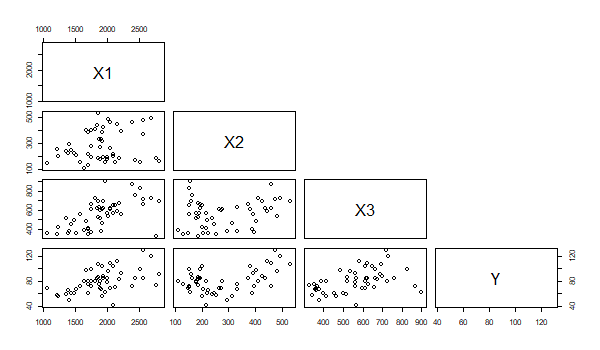
\includegraphics[width=.85\textwidth]{1.corr_plot_all_vars.png}
		\end{figure}
	The correlation matrix is also obtained, so the observations from the graph can be cross-check and validated by the correlation coefficents.
		\lstinputlisting[language=R, firstline=84, lastline=84]{PS1_answers_Duc Minh, Vu.R}
		\begin{verbatim}
			           Y        X1        X2        X3
			Y  1.0000000 0.5317212 0.4482876 0.4636787
			X1 0.5317212 1.0000000 0.2056101 0.5952504
			X2 0.4482876 0.2056101 1.0000000 0.2210149
			X3 0.4636787 0.5952504 0.2210149 1.0000000
		\end{verbatim}
		
	\begin{enumerate}
		\item The relationship between Y and X1
			\lstinputlisting[language=R, firstline=90, lastline=93]{PS1_answers_Duc Minh, Vu.R}
		Figure 2 displays the relationship between Per capita expenditure on housing assistance (Y) on the y-axis and Per capita income (X1) on the x-axis. 
			\begin{figure}[H]\centering
				\caption{\footnotesize Scatterplot between Y and X1.}
				\label{fig:plot_1}
				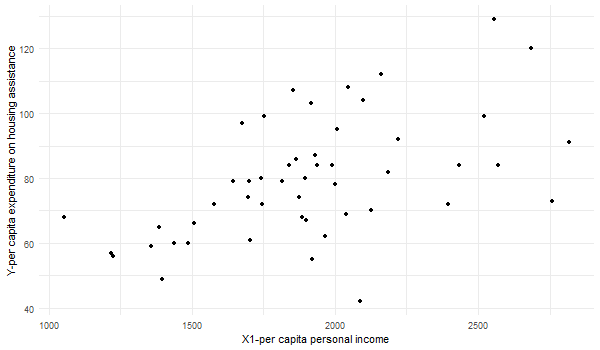
\includegraphics[width=.85\textwidth]{1.1.corr_plot_Y_and_X1.png}
			\end{figure}
		Visually, there is positive and linear relationship of weak-moderate strength between the two variables, in which Y tends to increase as X1 increases with a few potential outliers. So as Per capita income increases, Per capita expenditure also increases. This is confirmed by a moderate positive correlation coefficient of  r = 0.53 from the above correlation matrix.
		
		\item The relationship between Y and X2
			\lstinputlisting[language=R, firstline=100, lastline=103]{PS1_answers_Duc Minh, Vu.R}
		Figure 3 displays the relationship between Per capita expenditure on housing assistance (Y) on the y-axis and Number of residents per 100,000 that are "financially insecure" (X2) on the x-axis.
		\begin{figure}[H]\centering
			\caption{\footnotesize Scatterplot between Y and X2.}
			\label{fig:plot_1}
			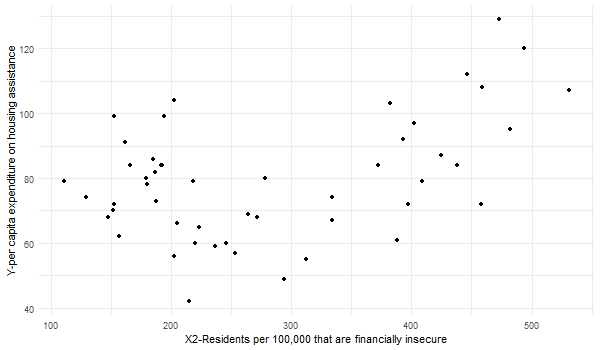
\includegraphics[width=.85\textwidth]{1.2.corr_plot_Y_and_X2.png}
		\end{figure}
		There seems to be a weak, positive and non-linear relationship between Y and X2. Per capita expenditure decrease up until around 300 residents per 100,000 before rising up again, which forms a U-shape concave up relationship. This is confirmed by a weak positive correlation coefficient of r = 0.45.
		
		\item The relationship between Y and X3
			\lstinputlisting[language=R, firstline=110, lastline=113]{PS1_answers_Duc Minh, Vu.R}
		Figure 4 displays the relationship between Per capita expenditure on housing assistance (Y) on the y-axis and Number of people per thousand residing in urban areas (X3) on the x-axis.
		\begin{figure}[H]\centering
			\caption{\footnotesize Scatterplot between Y and X3.}
			\label{fig:plot_1}
			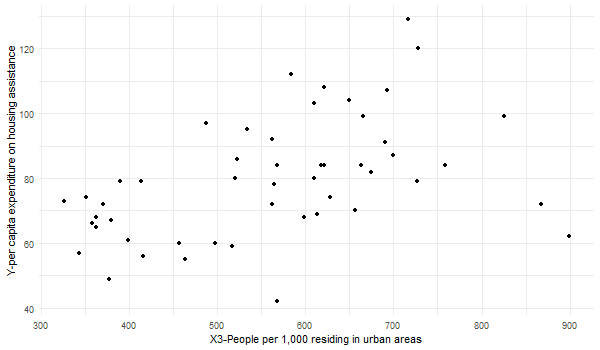
\includegraphics[width=.85\textwidth]{1.3.corr_plot_Y_and_X3.png}
		\end{figure}
		From the graph, we can observe a weak, positive and linear relationship between Y and X3, in which Y increases as X3 increases. This is confirmed  by a weak positive correlation coefficient of 0.46. Moreover, there seems to be a presence of clusters in this scatter plot, with X3 = 500 (people per 1,000) as the dividing line. There is a cluster of urban areas with low level of people residing (smaller than 500 per 1,000), and a cluster of urban areas with high level of people residing (larger than 500 per 1,000).
		
		\item The relationship between X1 and X2
			\lstinputlisting[language=R, firstline=120, lastline=123]{PS1_answers_Duc Minh, Vu.R}
		Figure 5 displays the relationship between Per capita income (X1) on the y-axis and Number of residents per 100,000 that are "financially insecure" (X2) on the x-axis.
		\begin{figure}[H]\centering
			\caption{\footnotesize Scatterplot between X1 and X2.}
			\label{fig:plot_1}
			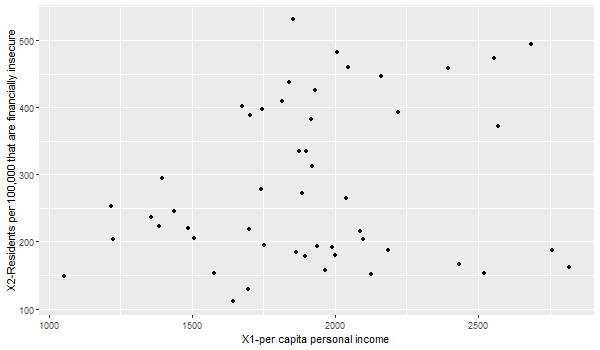
\includegraphics[width=.85\textwidth]{1.4.corr_plot_X1_and_X2.png}
		\end{figure}
		There is no clear direction for the points in this scatter plot, and no linear relationship can be detected. As such, there is no clear relationship between X1 and X2. This is confirmed by a very weak correaltion coefficient of 0.21.
		
		\item The relationship between X1 and X3
			\lstinputlisting[language=R, firstline=130, lastline=133]{PS1_answers_Duc Minh, Vu.R}
		Figure 6 displays the relationship between Per capita income (X1) on the y-axis and Number of people per thousand residing in urban areas (X3) on the x-axis.
		\begin{figure}[H]\centering
			\caption{\footnotesize Scatterplot between X1 and X3.}
			\label{fig:plot_1}
			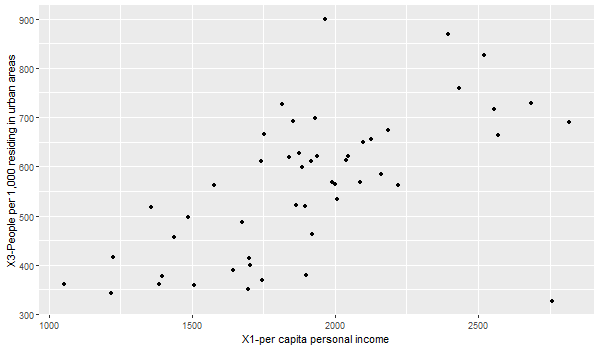
\includegraphics[width=.85\textwidth]{1.5.corr_plot_X1_and_X3.png}
		\end{figure}
		A positive, linear relationship of moderate strength can be depicted from Figure 6, as X1 increases when X3 increases with some potential outliers. So, people with higher capita income in a state tend to live more in the urban areas of that state. This relationship is confirmed by a moderate correlation coefficient of 0.59. Some potential clusters are also observed in this scatter plot, with 3 groups. The most visible group is state with "high" (in relation to this dataset) capita income, which is above \$2,250 threshold. The seperation between the "middle" and "low" income group is less visible, with \$1,750 as the separation line between these two clusters.
		
		\item The relationship between X2 and X3
			\lstinputlisting[language=R, firstline=140, lastline=143]{PS1_answers_Duc Minh, Vu.R}
		Figure 7 displays the relationship between Number of residents per 100,000 that are "financially insecure" (X2) on the y-axis and Number of people per thousand residing in urban areas (X3) on the x-axis.
		\begin{figure}[H]\centering
			\caption{\footnotesize Scatterplot between X2 and X3.}
			\label{fig:plot_1}
			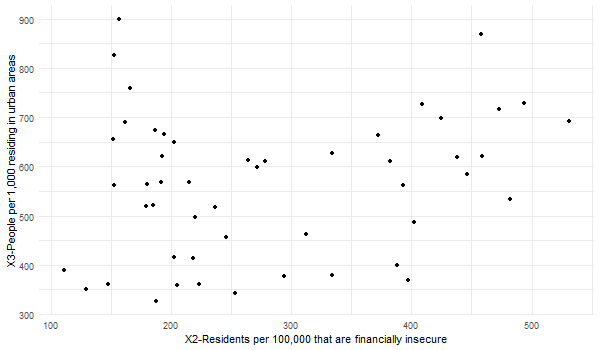
\includegraphics[width=.85\textwidth]{1.6.corr_plot_X2_and_X3.png}
		\end{figure}
		There is no clear relationship between X2 and X3 from this scatter plot which is confirmed by a low correlation coefficient of 0.221.

	\end{enumerate}
	\item \textbf{The relationships between Y and different regions} \\
	\lstinputlisting[language=R, firstline=148, lastline=152]{PS1_answers_Duc Minh, Vu.R}
	\lstinputlisting[language=R, firstline=157, lastline=169]{PS1_answers_Duc Minh, Vu.R}
	Figure 8 displays the relationship between Y and different regions of states in the US in the form of a box plot which shows the distribution of per capita spending expenditure according to each region. The average per capita spending is also calculated and depicted as the symbol "x' in the plot.
	
	\begin{figure}[H]\centering
		\caption{\footnotesize Box plot between Y and different Regions.}
		\label{fig:plot_1}
		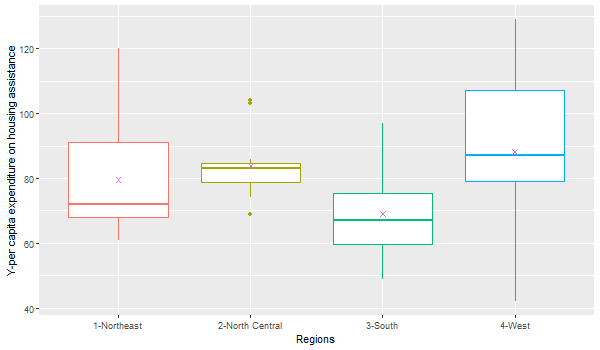
\includegraphics[width=.85\textwidth]{2.corr_plot_Y_and_Region.png}
	\end{figure}
		\lstinputlisting[language=R, firstline=172, lastline=175]{PS1_answers_Duc Minh, Vu.R}
	\begin{verbatim}
Region Region_name     ave_per_capita max_per_cap min_per_cap
<int> <chr>                    <dbl>       <int>       <int>
1      1 1-Northeast               79.4         120          61
2      2 2-North Central           83.9         104          69
3      3 3-South                   69.2          97          49
4      4 4-West                    88.3         129          42
	\end{verbatim}
	From the figure, we can then see that states in the \textbf{West} has the highest average above the three other states. This is confirmed by the calculated statistic as it has the highest mean for the per capita spending expenditure on housing assistance of 88.3.
	
	\vspace{1cm}
	
	\item \textbf{The relationships between Y and X1 with the inclusion of region}
		\lstinputlisting[language=R, firstline=191, lastline=199]{PS1_answers_Duc Minh, Vu.R}
	As described earlier in section 1.(a) of this question, Y and X1 as a weak-moderate positve and linear relationship, in which the higher the per capita income in a state, the more that state will spend on its housing assistance per capita. 
	\begin{figure}[H]\centering
		\caption{\footnotesize Scatterplot between Y and X1 for different regions.}
		\label{fig:plot_1}
		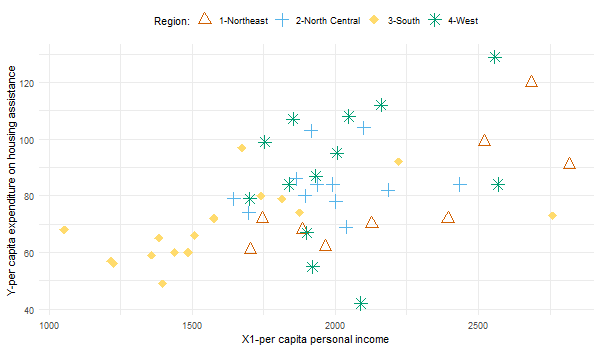
\includegraphics[width=.85\textwidth]{3.corr_plot_Y_and_X1_and_Region.png}
	\end{figure}
\end{enumerate} 
	With the inclusion of data on states' regions, we can then see how the relationships between Y and X1 differs for each region. For example: the linear positive relationship can be observerd more clearly for the South and Northeast regions, while no clear relationship can be seen for North Central and West regions. 
\end{document}